% Block diagram of the pipelined NICE core, rendered to pipeline.png by
% "make diagrams" in the top-level Makefile. MICROARCH.md §3 shows it.
% Edit this file, not the PNG, and render again when the entities change.
%
% What it shows: the four stages in pipeline order, the data bus port DBUS
% beside PREPARE and WRITE, the two Wishbone buses leaving on the right,
% and the dotted boundary of the top level, pipeline. Each block is the
% VHDL entity of its name, hdl/src/pipe_fetch.vhd for FETCH and so on. The
% thin arrows on the left are the paths that are not the main flow: the
% flush and redirect from WRITE, the early redirect from DECODE, and
% PREPARE's reads of the registers that WRITE holds. It does not show the
% handshakes, the interrupt ports, or the trace report.
%
% The short black bars are the registers on the main path. Each is drawn
% inside the block of the entity that holds it, at the edge where its
% value comes in or leaves:
%
%   FETCH, on the instruction address          req_r and stb_r (pipe_fetch)
%   FETCH, at its output                       ring_r (pipe_fetch)
%   DECODE, between taking an instruction      dec_r, and dec_q, the
%     and splitting it                           instruction after it, which
%                                              waits there (pipe_decode)
%   PREPARE, at its input                      prep_r (pipe_prepare)
%   PREPARE, on its read request               rd_stb_r, rd_addr_r (pipe_prepare)
%   DBUS, on WRITE's store                     st_r (pipe_dbus)
%   WRITE, at its input                        w_r.uop (pipe_write)
%
% So no register sits between two blocks: the words from ring_r reach
% dec_r, the micro-operation from dec_r reaches prep_r, and the one from
% prep_r reaches w_r.uop, each through logic only. WRITE's store goes
% into a register in DBUS, st_r, which drives the bus in the next cycle.
% Read data that only goes into a register reaches WRITE in the cycle its
% ACK comes, past DBUS's FIFO. Other read data comes from the FIFO.

\documentclass[border=8pt]{standalone}

\usepackage[T1]{fontenc}
\usepackage{helvet}
\renewcommand{\familydefault}{\sfdefault}

\usepackage{tikz}
\usetikzlibrary{arrows.meta, positioning, fit, calc}

\begin{document}

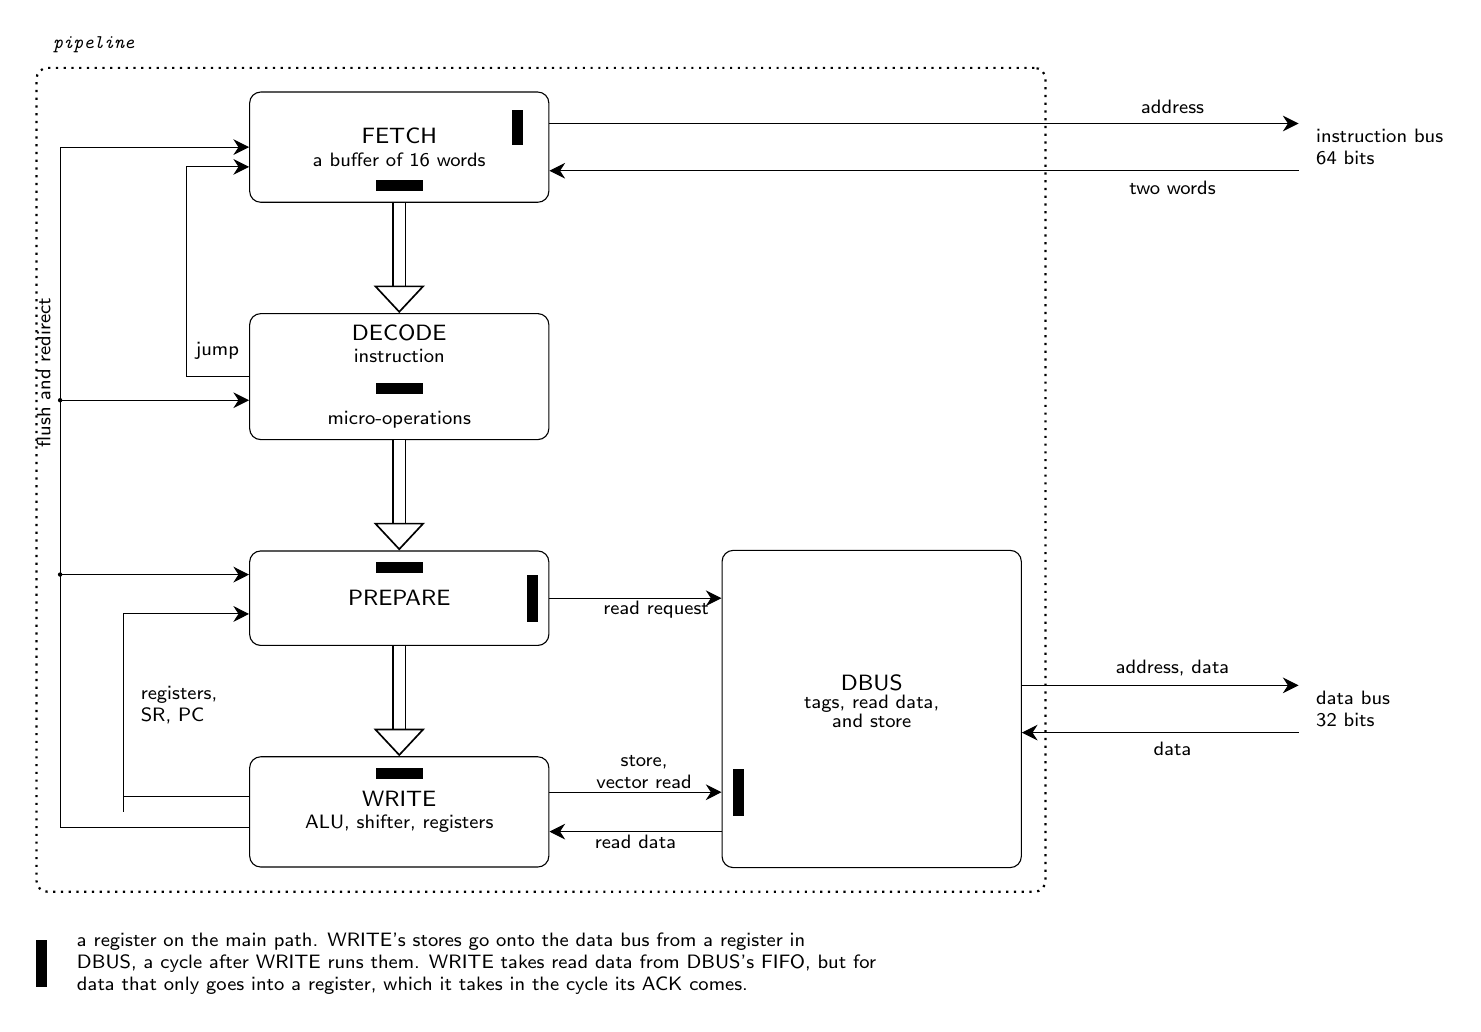
\begin{tikzpicture}[
      font = \sffamily\footnotesize,
      % A part of the pipeline, one VHDL entity
      block/.style = {
         draw,
         rounded corners = 4pt,
         minimum width   = 38mm,
         minimum height  = 10mm,
         align           = center
      },
      % The main flow: one instruction or micro-operation per beat. The line
      % width stays at 0.5pt or more, so that both slivers of the doubled
      % line survive the 150 dpi rendering.
      flow/.style = {
         draw,
         line width      = 0.6pt,
         double,
         double distance = 4pt,
         -{Triangle[open, length = 3.5mm, width = 6.5mm]}
      },
      wire/.style     = {draw, -{Stealth[length = 2mm, width = 2mm]}},
      buslabel/.style = {midway, font = \sffamily\scriptsize, inner sep = 1pt},
      wirelabel/.style = {font = \sffamily\scriptsize, align = center},
      % A label placed by itself, not on a path
      looselabel/.style = {font = \sffamily\scriptsize},
      % A register on the main path, drawn across the path it cuts: ffh for
      % vertical arrows, ffv for horizontal ones.
      ffh/.style = {fill = black, inner sep = 0pt,
                    minimum width = 6mm, minimum height = 1.4mm},
      ffv/.style = {fill = black, inner sep = 0pt,
                    minimum width = 1.4mm, minimum height = 6mm}
   ]

   %% ---------------------------------------------------------------
   %% The stages, top to bottom
   %% ---------------------------------------------------------------

   \node[block, minimum height = 14mm]    (fetch)   {FETCH\\[-0.5mm]
                                                     {\scriptsize a buffer of 16 words}};
   \node[block, below = 14mm of fetch,
         minimum height = 16mm]           (decode)  {DECODE\\[-0.5mm]
                                                     {\scriptsize instruction}\\[4.5mm]
                                                     {\scriptsize micro-operations}};
   \node[block, below = 14mm of decode,
         minimum height = 12mm]           (prepare) {PREPARE};
   \node[block, below = 14mm of prepare,
         minimum height = 14mm]           (write)   {WRITE\\[-0.5mm]
                                                     {\scriptsize ALU, shifter, registers}};

   \draw[flow] (fetch)   -- (decode);
   \draw[flow] (decode)  -- (prepare);
   \draw[flow] (prepare) -- (write);

   %% ---------------------------------------------------------------
   %% The data bus port, beside PREPARE and WRITE
   %% ---------------------------------------------------------------

   \coordinate (dbusx) at ([xshift = 60mm] prepare.center);
   \node[block, inner sep = 0pt,
         fit = {([xshift = -14mm] dbusx |- prepare.north)
                ([xshift =  14mm] dbusx |- write.south)}] (dbus) {DBUS\\[-0.5mm]
                {\scriptsize tags, read data,\\[-1mm] \scriptsize and store}};

   % PREPARE's read requests and WRITE's stores go out through it; the read
   % data comes back to WRITE.
   \draw[wire] (prepare.east) -- (dbus.west |- prepare.east)
      node[buslabel, below, pos = 0.62] {read request};
   \draw[wire] ([yshift = 2.5mm] write.east) -- ([yshift = 2.5mm] dbus.west |- write.east)
      node[buslabel, above, pos = 0.55, align = center] {store,\\ vector read};
   \draw[wire] ([yshift = -2.5mm] dbus.west |- write.east) -- ([yshift = -2.5mm] write.east)
      node[buslabel, below] {read data};

   %% ---------------------------------------------------------------
   %% The paths on the left
   %% ---------------------------------------------------------------

   % PREPARE reads the registers that WRITE holds, for the address of a
   % data read.
   \coordinate (regsx) at ([xshift = -24mm] write.west);
   \draw[wire] ([yshift = 2mm] write.west) -| ([xshift = 8mm] regsx)
      |- ([yshift = -2mm] prepare.west);
   \node[wirelabel, anchor = west, align = left]
      at ($ ([xshift = 9mm] regsx |- prepare.west)!0.5!([xshift = 9mm] regsx |- write.west) $)
      {registers,\\ SR, PC};

   % The flush and redirect from WRITE, to every stage, and the early
   % redirect from DECODE, to FETCH. The branches to DECODE and PREPARE
   % pass below the jump and above the registers, so no lines cross.
   \draw[wire] ([yshift = -2mm] write.west) -| (regsx) |- (fetch.west);
   \coordinate (flushd) at ([yshift = -3mm] decode.west);
   \coordinate (flushp) at ([yshift =  3mm] prepare.west);
   \draw[wire] (regsx |- flushd) -- (flushd);
   \draw[wire] (regsx |- flushp) -- (flushp);
   \fill (regsx |- flushd) circle (0.8pt);
   \fill (regsx |- flushp) circle (0.8pt);
   \node[wirelabel, anchor = south, rotate = 90]
      at ($ (regsx |- fetch.west)!0.5!(regsx |- prepare.west) $) {flush and redirect};
   \draw[wire] (decode.west) -- ([xshift = -8mm] decode.west) |- ([yshift = -2.5mm] fetch.west);
   \node[wirelabel, anchor = south west] at ([xshift = -8mm, yshift = 1mm] decode.west)
      {jump};

   %% ---------------------------------------------------------------
   %% The top level
   %% ---------------------------------------------------------------

   \node[draw, dotted, thick, rounded corners = 4pt, inner sep = 3mm,
         fit = (fetch) (decode) (prepare) (write) (dbus) (regsx)] (top) {};
   \node[anchor = south west, font = \ttfamily\scriptsize\itshape]
      at ([xshift = 1mm, yshift = 0.5mm] top.north west) {pipeline};

   %% ---------------------------------------------------------------
   %% The two Wishbone buses
   %% ---------------------------------------------------------------

   % The labels sit on the part of each bus outside the top level.
   \coordinate (busx)  at ([xshift = 32mm] top.east);
   \coordinate (ibusl) at (fetch.east);
   \coordinate (ibusr) at (busx |- fetch.east);
   \coordinate (dbusl) at (dbus.east);
   \coordinate (dbusr) at (busx |- dbus.east);
   \coordinate (ibusm) at ($ (top.east |- ibusl)!0.5!(ibusr) $);
   \coordinate (dbusm) at ($ (top.east |- dbusl)!0.5!(dbusr) $);

   \draw[wire] ([yshift =  3mm] ibusl) -- ([yshift =  3mm] ibusr);
   \draw[wire] ([yshift = -3mm] ibusr) -- ([yshift = -3mm] ibusl);
   \node[looselabel, above] at ([yshift =  3mm] ibusm) {address};
   \node[looselabel, below] at ([yshift = -3mm] ibusm) {two words};

   \draw[wire] ([yshift =  3mm] dbusl) -- ([yshift =  3mm] dbusr);
   \draw[wire] ([yshift = -3mm] dbusr) -- ([yshift = -3mm] dbusl);
   \node[looselabel, above] at ([yshift =  3mm] dbusm) {address, data};
   \node[looselabel, below] at ([yshift = -3mm] dbusm) {data};

   \node[font = \sffamily\scriptsize, anchor = west, align = left] at ([xshift = 1mm] ibusr)
      {instruction bus\\64 bits};
   \node[font = \sffamily\scriptsize, anchor = west, align = left] at ([xshift = 1mm] dbusr)
      {data bus\\32 bits};

   %% ---------------------------------------------------------------
   %% The registers on the main path
   %% ---------------------------------------------------------------
   %
   % Drawn last, on top of the arrows they cut. See the header.

   % FETCH's request, at the base of the instruction address arrow
   \node[ffv, minimum height = 4.5mm] at ([xshift = -4mm, yshift = 2.5mm] fetch.east) {};

   % FETCH's ring, at the bottom of its block, DECODE's dec_r, between the
   % instruction it takes and the micro-operations it emits, and PREPARE's
   % prep_r and WRITE's w_r.uop, at the top of theirs
   \node[ffh] at ([yshift = 2.2mm] fetch.south) {};
   \node[ffh] at ([yshift = -1.5mm] decode.center) {};
   \node[ffh] at ([yshift = -2.2mm] prepare.north) {};
   \node[ffh] at ([yshift = -2.2mm] write.north) {};

   % PREPARE's read request, at the right of its block, and DBUS's store
   % register, at the left of its block
   \node[ffv] at ([xshift = -2.2mm] prepare.east) {};
   \node[ffv] at ([xshift = 2.2mm, yshift = 2.5mm] dbus.west |- write.east) {};

   %% ---------------------------------------------------------------
   %% Legend
   %% ---------------------------------------------------------------

   \node[ffv, anchor = west] (legendff) at ([yshift = -9mm] top.south west) {};
   \node[anchor = west, font = \sffamily\scriptsize, align = left]
      at ([xshift = 2.5mm] legendff.east)
      {a register on the main path. WRITE's stores go onto the data bus from a register in\\
       DBUS, a cycle after WRITE runs them. WRITE takes read data from DBUS's FIFO, but for\\
       data that only goes into a register, which it takes in the cycle its ACK comes.};

\end{tikzpicture}

\end{document}
